% AutoPareto poster -- DRAFT (NeurIPS 2026 AutoMLR workshop).  Build: cd paper/camera_ready/poster && tectonic poster.tex
% Size is a placeholder (A0 landscape); change \geometry once the workshop's poster size is confirmed.
% Every number comes from the camera-ready macros (analysis/cr_tables.py, analysis/cr_v2.py).
\documentclass{article}
\usepackage[paperwidth=46.8in,paperheight=33.1in,margin=1.1in]{geometry}
\usepackage[T1]{fontenc}
\usepackage{lmodern}
\usepackage{graphicx,xcolor,booktabs,amsmath}
\usepackage[most]{tcolorbox}
% Generated by analysis/cr_tables.py from paper/camera_ready/data/cr_stats.json. Do not edit by hand.
\newcommand{\CRDecodeRatio}{1.99}
\newcommand{\CRDecodeRatioSeeds}{1.97, 1.96, 2.03}
\newcommand{\CRDecodeRatioMin}{1.96}
\newcommand{\CRDecodeRatioMax}{2.03}
\newcommand{\CRParamReduction}{41.7}
\newcommand{\CRMemoryReduction}{35.1}
\newcommand{\CRAPQSpeed}{383.0}
\newcommand{\CRARSpeed}{192.9}
\newcommand{\CRAPQHeld}{1.1418}
\newcommand{\CRARHeld}{1.0998}
\newcommand{\CRAPQParams}{29.36}
\newcommand{\CRARParams}{50.33}
\newcommand{\CRAPQMem}{162.9}
\newcommand{\CRARMem}{250.9}
\newcommand{\CRAPQKV}{1.992}
\newcommand{\CRARKV}{3.984}
\newcommand{\CRHeldDiff}{+0.042}
\newcommand{\CRHeldDiffAbs}{0.042}
\newcommand{\CRHeldDiffFour}{+0.0420}
\newcommand{\CRHeldCI}{[+0.030, +0.054]}
\newcommand{\CRHeldCIFour}{[+0.0297, +0.0544]}
\newcommand{\CRHeldCILo}{0.030}
\newcommand{\CRHeldCIHi}{0.054}
\newcommand{\CRValDiff}{+0.045}
\newcommand{\CRValDiffFour}{+0.0451}
\newcommand{\CRValCIFour}{[+0.0415, +0.0486]}
\newcommand{\CRHeldSeeds}{+0.0387, +0.0477, +0.0397}
\newcommand{\CRValSeeds}{+0.0440, +0.0467, +0.0445}
\newcommand{\CRFixedDiff}{$-$0.0067}
\newcommand{\CRFixedDiffThree}{$-$0.007}
\newcommand{\CRFixedCIFour}{[$-$0.0130, $-$0.0003]}
\newcommand{\CRFixedSeeds}{$-$0.0054, $-$0.0051, $-$0.0096}
\newcommand{\CRDiscGap}{$-$0.0017}
\newcommand{\CRPooledSD}{0.0022}
\newcommand{\CRMaxHeldSD}{0.0060}
\newcommand{\CRBaseSeedEffect}{0.024}
\newcommand{\CRSeedFortyTwoAP}{1.0940}
\newcommand{\CRSeedFortyTwoAR}{1.0950}
\newcommand{\CRSeedFortyTwoTPE}{1.0977}
\newcommand{\CRSeedFortyTwoMOTPE}{1.0981}
\newcommand{\CRSeedFortyTwoSpread}{0.0041}
\newcommand{\CROptMin}{0.0014}
\newcommand{\CROptMax}{0.0087}
\newcommand{\CRGapTwoMax}{0.0003}
\newcommand{\CRGapFiveMax}{0.0021}
\newcommand{\CRTokenSpreadMax}{18.7}
\newcommand{\CRExpOneThreeSixDisc}{251.8}
\newcommand{\CRExpOneThreeSixRerunLo}{209.7}
\newcommand{\CRExpOneThreeSixRerunHi}{220.5}
\newcommand{\CRExpOneZeroNineBPB}{1.0940}
\newcommand{\CRExpOneZeroNineTokens}{84.1}
\newcommand{\CRExpSixEightTokens}{88.9}
\newcommand{\CRAPAttempts}{75}
\newcommand{\CRCatArch}{32}
\newcommand{\CRCatOptimizer}{21}
\newcommand{\CRCatOptimization}{10}
\newcommand{\CRCatBatching}{8}
\newcommand{\CRCatSchedule}{4}
\newcommand{\CRStepNineteenTwenty}{0.0020}
\newcommand{\CRStepTwentyTwentyTwo}{0.00009}
\newcommand{\CRAnineBPB}{1.1068}
\newcommand{\CRAtenBPB}{1.1054}
\newcommand{\CRAnineDec}{324.7}
\newcommand{\CRAtenDec}{291.0}
\newcommand{\CRAtwentyfiveDec}{408.4}
\newcommand{\CRFrontierN}{6}
\newcommand{\CRPanelBudget}{201{,}326{,}592}
\newcommand{\CRARTokRatio}{2.28}
\newcommand{\CRAPQTokRatio}{1.28}
\newcommand{\CRFixedSixtyFive}{1.1017}
\newcommand{\CRFixedSixtyEight}{1.1014}
\newcommand{\CRBLiMPLower}{51}
\newcommand{\CRBLiMPTied}{1}
\newcommand{\CRBLiMPHigher}{15}
\newcommand{\CRBLiMPConfigs}{67}
\newcommand{\CRNCrossChecked}{118}
\newcommand{\CRSessionLo}{0.0035}
\newcommand{\CRSessionHi}{0.0070}
\newcommand{\CRHeldValOffLo}{0.053}
\newcommand{\CRHeldValOffHi}{0.069}
\newcommand{\CRCorrBLiMPHeld}{-0.969}
\newcommand{\CRCorrBLiMPDepth}{0.717}
\newcommand{\CRAPQARCE}{36.91}
\newcommand{\CRAPQPIQA}{58.29}
\newcommand{\CRAPQLAMBADA}{21.50}
\newcommand{\CRAPQBLiMP}{72.02}
\newcommand{\CRARARCE}{36.50}
\newcommand{\CRARPIQA}{58.67}
\newcommand{\CRARLAMBADA}{20.44}
\newcommand{\CRARBLiMP}{74.56}
\newcommand{\CRARCESE}{1.0}

% Generated by analysis/cr_v2.py from paper/camera_ready/data/cr_v2.json. Do not edit by hand.
\newcommand{\CREOneHeldA}{+0.0385}
\newcommand{\CREOneHeldB}{+0.0396}
\newcommand{\CREOneHeldC}{+0.0415}
\newcommand{\CREOneMatchedLo}{+0.038}
\newcommand{\CREOneMatchedHi}{+0.042}
\newcommand{\CREOneMatchedLoAbs}{0.038}
\newcommand{\CREOneMatchedHiAbs}{0.042}
\newcommand{\CREOneTimeHeld}{$-$0.0022}
\newcommand{\CREOneTimeHeldThree}{$-$0.002}
\newcommand{\CREOneTimeHeldCI}{[$-$0.020, +0.016]}
\newcommand{\CREOneTimeHeldLo}{$-$0.020}
\newcommand{\CREOneTimeHeldHi}{+0.016}
\newcommand{\CREOneTimeVal}{$-$0.0044}
\newcommand{\CREOneTimeValThree}{$-$0.004}
\newcommand{\CREOneTimeValCI}{[$-$0.012, +0.004]}
\newcommand{\CREOneTimeHeldWins}{1}
\newcommand{\CREOneContrast}{+0.0031}
\newcommand{\CREOneContrastCI}{[$-$0.0017, +0.0078]}
\newcommand{\CREOnePairs}{9}
\newcommand{\CREOneMaxSD}{0.0045}
\newcommand{\CREOneReplDiff}{$-$0.0005}
\newcommand{\CREOneReplCI}{[$-$0.0120, +0.0110]}
\newcommand{\CREOneTokAP}{158.1}
\newcommand{\CREOneTokAR}{88.0}
\newcommand{\CREOneTokRatio}{1.80}
\newcommand{\CREOneHistWelch}{+0.0023}
\newcommand{\CREOneResamples}{27}
\newcommand{\CREOneExposure}{$-$0.041}
\newcommand{\CREOneExposureCI}{[$-$0.042, $-$0.039]}
\newcommand{\CREOneArch}{+0.040}
\newcommand{\CREOneArchCI}{[+0.023, +0.056]}
\newcommand{\CREOneSched}{$-$0.001}
\newcommand{\CREOneExposureVal}{$-$0.047}
\newcommand{\CREOneArchVal}{+0.043}
\newcommand{\CREOneRho}{1.81}
\newcommand{\CREOneK}{1.79}
\newcommand{\CREOneKCI}{[1.29, 2.28]}
\newcommand{\CREOneKVal}{1.70}
\newcommand{\CRFixedTokAR}{88.5}
\newcommand{\CRFixedTokAPQ}{156.9}
\newcommand{\CRAgBaseBPB}{1.1999}
\newcommand{\CRAgBaseTok}{85.5}
\newcommand{\CRAgBaseMem}{337}
\newcommand{\CRAgBaseDecode}{149}
\newcommand{\CRAgEtoERef}{146}
\newcommand{\CRAgEtoERefRep}{143}
\newcommand{\CRAgPrefillRef}{7.5}
\newcommand{\CROpStableRepeats}{6}
\newcommand{\CROpRepeats}{9}
\newcommand{\CROpAttempts}{27}
\newcommand{\CROpValid}{25}
\newcommand{\CROpValidFrozen}{23}
\newcommand{\CROpUncertain}{7}
\newcommand{\CROpBestBPB}{1.0962}
\newcommand{\CROpBestAttempt}{23}
\newcommand{\CROpBestFrozen}{1.0962}
\newcommand{\CROpBestTwentyTwo}{1.0969}
\newcommand{\CROpBestTwentyTwoAttempt}{20}
\newcommand{\CROpBestSeven}{1.0995}
\newcommand{\CROpLateGain}{0.0033}
\newcommand{\CROpUpdLo}{1,504}
\newcommand{\CROpUpdHi}{1,514}
\newcommand{\CROpLateDone}{19}
\newcommand{\CROpLateInf}{11}
\newcommand{\CROpMaxTok}{232}
\newcommand{\CROpTokLo}{197}
\newcommand{\CROpTokHi}{198}
\newcommand{\CROpTokRatio}{2.3}
\newcommand{\CROpDecodeLo}{30.9}
\newcommand{\CROpDecodeHi}{31.8}
\newcommand{\CROpEtoELo}{5.2}
\newcommand{\CROpEtoEHi}{5.3}
\newcommand{\CROpPrefillLo}{140}
\newcommand{\CROpPrefillHi}{143}
\newcommand{\CROpMemLo}{97}
\newcommand{\CROpMemHi}{113}
\newcommand{\CROpHeldLo}{1.158}
\newcommand{\CROpHeldHi}{1.161}
\newcommand{\CROpARHeld}{1.100}
\newcommand{\CROpAPQHeld}{1.142}
\newcommand{\CROpTokFrac}{98}
\newcommand{\CROpAdapterAttempt}{10}
\newcommand{\CROpPreAdapterDecode}{2.6}
\newcommand{\CROpPreAdapterPrefill}{6}
\newcommand{\CROpAdapterDecode}{8.6}
\newcommand{\CROpAdapterPrefill}{81}
\newcommand{\CROpDLambadaLo}{+0.049}
\newcommand{\CROpDLambadaHi}{+0.061}
\newcommand{\CROpDBlimpLo}{+0.059}
\newcommand{\CROpDBlimpHi}{+0.070}
\newcommand{\CROpDHeldLo}{0.088}
\newcommand{\CROpDHeldHi}{0.091}
\newcommand{\CREOneHours}{4.76}
\newcommand{\CREOneTputAR}{288.2--289.7k}
\newcommand{\CREOneTputAP}{520.7--524.9k}
\newcommand{\CREZeroTputAR}{287.0k}
\newcommand{\CREZeroTputAP}{521.8k}
\newcommand{\CROpFrontierFrozen}{A21, A23, A24}
\newcommand{\CROpFrontierExtended}{A23, A24, A27}
\newcommand{\CRCxAttempts}{22}
\newcommand{\CRCxValid}{22}
\newcommand{\CRCxUncertain}{1}
\newcommand{\CRCxBestBPB}{1.1016}
\newcommand{\CRCxBestAttempt}{14}
\newcommand{\CRCxBestTok}{126.6}
\newcommand{\CRCxMaxTok}{175}
\newcommand{\CRCxBestDecode}{1.32}
\newcommand{\CRCxMaxDecode}{1.58}
\newcommand{\CRCxMaxPrefill}{27}
\newcommand{\CRMTRuns}{10}
\newcommand{\CRMTPairs}{9}
\newcommand{\CRMTDLo}{+0.059}
\newcommand{\CRMTDHi}{+0.061}
\newcommand{\CRMTDLoAbs}{0.059}
\newcommand{\CRMTDHiAbs}{0.061}
\newcommand{\CRMTCIMin}{+0.051}
\newcommand{\CRMTHolm}{0.002}
\newcommand{\CRMTDAPLo}{+0.017}
\newcommand{\CRMTDAPHi}{+0.019}
\newcommand{\CRMTDAPCIMin}{+0.004}
\newcommand{\CRMTValLo}{+0.062}
\newcommand{\CRMTValHi}{+0.065}
\newcommand{\CRMTHeldLo}{1.158}
\newcommand{\CRMTHeldHi}{1.160}
\newcommand{\CRMTARHeld}{1.099}
\newcommand{\CRMTAPHeld}{1.141}
\newcommand{\CRMTTpsLo}{657}
\newcommand{\CRMTTpsHi}{658}
\newcommand{\CRMTTpsAR}{289}
\newcommand{\CRMTTpsAP}{523}
\newcommand{\CRMTRhoLo}{2.27}
\newcommand{\CRMTRhoHi}{2.28}
\newcommand{\CRMTKBound}{2.27}
\newcommand{\CRMTKExtLo}{2.38}
\newcommand{\CRMTKExtHi}{2.46}
\newcommand{\CRMTPostLo}{+0.001}
\newcommand{\CRMTPostHi}{+0.003}
\newcommand{\CRMTPostCILo}{$-$0.005}
\newcommand{\CRMTPostCIHi}{+0.012}
\newcommand{\CRMTBlimpLo}{0.034}
\newcommand{\CRMTBlimpHi}{0.038}
\newcommand{\CRMTBlimpLoPts}{3.4}
\newcommand{\CRMTBlimpHiPts}{3.8}
\newcommand{\CRMTKAPQ}{1.86}
\newcommand{\CRMTDrift}{$-$0.0010}
\newcommand{\CRMTDriftAbs}{0.0010}
\newcommand{\CRMTParamsLo}{22.0}
\newcommand{\CRMTParamsHi}{26.2}
\newcommand{\CRIARuns}{39}
\newcommand{\CRIAUnstable}{5}
\newcommand{\CRIATotalLo}{30.7}
\newcommand{\CRIATotalHi}{30.8}
\newcommand{\CRIAGraphLo}{11.2}
\newcommand{\CRIAGraphHi}{11.7}
\newcommand{\CRIAFusionLo}{2.7}
\newcommand{\CRIAFusionHi}{2.8}
\newcommand{\CRIAJointLo}{15.6}
\newcommand{\CRIAJointHi}{16.7}
\newcommand{\CRIAInteractLo}{0.51}
\newcommand{\CRIAInteractHi}{0.52}
\newcommand{\CRIAAttnLo}{1.29}
\newcommand{\CRIAAttnHi}{1.29}
\newcommand{\CRIARingLo}{1.05}
\newcommand{\CRIARingHi}{1.05}
\newcommand{\CRIAArchLo}{1.85}
\newcommand{\CRIAArchHi}{1.97}
\newcommand{\CRIATotalMed}{31}
\newcommand{\CRIAEtoEMed}{5.3}
\newcommand{\CRIAEtoELo}{5.2}
\newcommand{\CRIAEtoEHi}{5.4}
\newcommand{\CRIAGraphEtoELo}{1.9}
\newcommand{\CRIAGraphEtoEHi}{2.0}
\newcommand{\CRIAFusionEtoEHi}{1.07}
\newcommand{\CRIAPrefillLo}{131}
\newcommand{\CRIAPrefillHi}{138}
\newcommand{\CRIAPrefillNGLo}{3.7}
\newcommand{\CRIAPrefillNGHi}{4.3}
\newcommand{\CRIAPrefillBase}{7.3}
\newcommand{\CRIACapture}{97}
\newcommand{\CRIAKVOp}{3.6}
\newcommand{\CRIAKVLin}{7.5}
\newcommand{\CRIABaseDecode}{149}
\newcommand{\CRIABaseDecodeLo}{145}
\newcommand{\CRIABaseDecodeHi}{153}
\newcommand{\CRIAKernBase}{625}
\newcommand{\CRIALaunchBase}{618}
\newcommand{\CRIAKernEager}{290}
\newcommand{\CRIAKernFused}{78}
\newcommand{\CRIALaunchNG}{75}
\newcommand{\CRIALaunchGraph}{2}
\newcommand{\CRMTHours}{2.61}
\newcommand{\CRIAHours}{3.10}
\newcommand{\CRBenchSDMax}{2.3}
\newcommand{\CRBenchSDMed}{0.7}

\pagestyle{empty}
\setlength{\parindent}{0pt}
\setlength{\parskip}{0.45em}
\definecolor{ink}{HTML}{0B0B0B}
\definecolor{ink2}{HTML}{52514E}
\definecolor{apq}{HTML}{2A78D6}
\definecolor{arref}{HTML}{EB6834}
\definecolor{opus}{HTML}{6250D6}
\definecolor{rule}{HTML}{D8D6D0}
\definecolor{todo}{HTML}{B2412A}
\newtcolorbox{panel}[1]{enhanced,breakable=false,colback=white,colframe=rule,boxrule=2pt,arc=6pt,
  left=22pt,right=22pt,top=16pt,bottom=18pt,fonttitle=\sffamily\bfseries\fontsize{40}{46}\selectfont,
  coltitle=ink,colbacktitle=white,title={#1},attach boxed title to top left={yshift=-8pt,xshift=14pt},
  boxed title style={colframe=white,colback=white}}
\newcommand{\statnum}[2]{{\color{#1}\sffamily\bfseries\fontsize{60}{66}\selectfont #2}}
\newcommand{\todo}[1]{{\color{todo}[#1]}}
\begin{document}
\fontsize{31}{39}\selectfont\color{ink}
% ---------------------------------------------------------------- header
\begin{minipage}[t]{0.82\linewidth}
{\sffamily\bfseries\fontsize{86}{96}\selectfont AutoPareto: what a fixed-time contract pays for}\\[18pt]
{\fontsize{40}{48}\selectfont Auditing autonomous Transformer search with matched-exposure verification}\\[14pt]
{\fontsize{34}{40}\selectfont Rami Alobaidy \quad \todo{affiliation} \quad rameonix@gmail.com}
\end{minipage}\hfill
\begin{minipage}[t]{0.17\linewidth}\raggedleft
{\sffamily\fontsize{28}{34}\selectfont NeurIPS 2026 Workshop for\\Autonomous ML Research\\[10pt]\todo{DRAFT: author to review}\\[6pt]\todo{QR code to paper/artifact}}
\end{minipage}

\vspace{22pt}{\color{rule}\rule{\linewidth}{3pt}}\vspace{18pt}

% ---------------------------------------------------------------- three columns
\begin{minipage}[t]{0.305\linewidth}\vspace{0pt}
\begin{panel}{The question}
Autonomous ML researchers are usually scored under a \textbf{fixed wall-clock budget}. A program that trains faster also sees more data before it is scored, so a discovery-stage score mixes the agent's edit with the tokens the contract hands it.

\textbf{Does the agent's winning recipe hold up when exposure is matched?}
\end{panel}
\vspace{18pt}
\begin{panel}{AutoPareto}
\raggedright An LLM agent edits one file, \texttt{train.py}; a hash-checked harness trains it for 300\,s on one A40 and scores validation BPB, cached-decode speed and peak memory. Failures stay in the lineage.\\[8pt]
\centering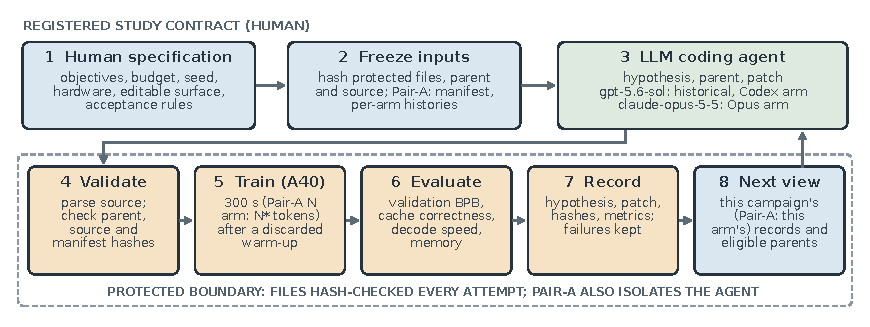
\includegraphics[width=\linewidth]{../poster_figures/research_loop.pdf}
\end{panel}
\vspace{18pt}
\begin{panel}{What the agent found}
\centering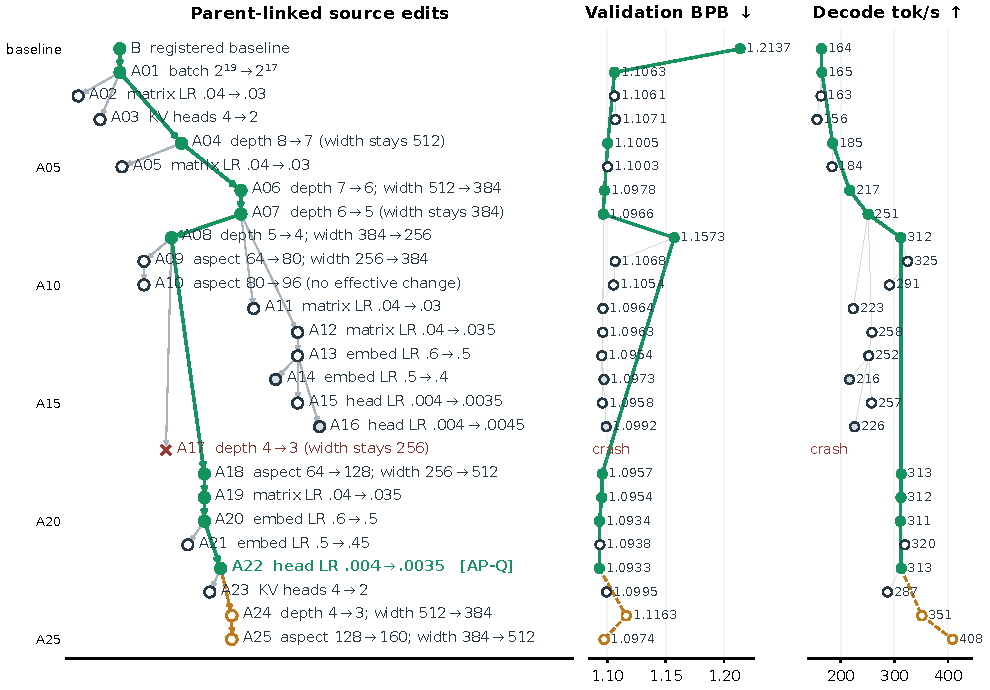
\includegraphics[width=0.86\linewidth]{../poster_figures/autopareto_lineage.pdf}\\[6pt]
\raggedright AP-Q halves AR-ref's depth (4 vs 8 layers) and trains \statnum{apq}{\CREOneRho$\times$} faster. Three recorded hypotheses on its path cite the extra tokens a cheaper model gets in 300\,s.
\end{panel}
\end{minipage}\hfill
% ---------------------------------------------------------------- column 2
\begin{minipage}[t]{0.37\linewidth}\vspace{0pt}
\begin{panel}{Pre-registered test (E1): tokens, not architecture}
\raggedright AP-Q (\textcolor{apq}{\textbf{blue}}) vs AR-ref (\textcolor{arref}{\textbf{orange}}) at three matched token budgets and at 300\,s, fresh seeds 6--8, 24 runs (plan committed before running).\\[8pt]
\centering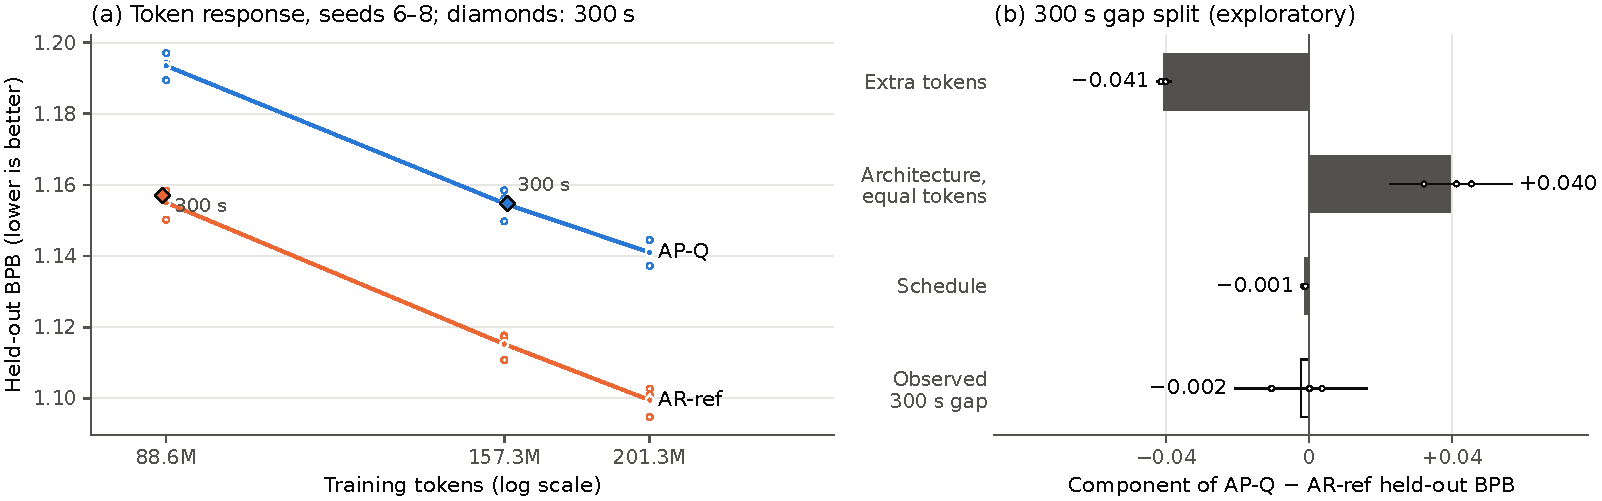
\includegraphics[width=\linewidth]{../poster_figures/cr_e1.pdf}\\[10pt]
\raggedright
\begin{tabular}{@{}lll@{}}
\toprule
& $\Delta$ held-out BPB (AP-Q $-$ AR-ref) & AP-Q better \\
\midrule
88.6M tokens & \CREOneHeldA & 0 of 3 seeds \\
157.3M tokens & \CREOneHeldB & 0 of 3 \\
201.3M tokens & \CREOneHeldC & 0 of 3 \\
300\,s (AP-Q: \CREOneTokRatio$\times$ tokens) & \CREOneTimeHeld{} \CREOneTimeHeldCI & \CREOneTimeHeldWins{} of 3 \\
\bottomrule
\end{tabular}\\[12pt]
\begin{itemize}\setlength{\itemsep}{4pt}
\item Worse at \textbf{every} matched budget, \CREOnePairs{} of 9 seed pairs; no crossover.
\item At 300\,s: a statistical \textbf{tie}.
\item Gap split: extra tokens \statnum{ink}{\CREOneExposure}, architecture \statnum{ink}{\CREOneArch}.
\item AP-Q needs $\approx$\CREOneK$\times$ AR-ref's tokens for equal quality, and trains \CREOneRho$\times$ faster.
\end{itemize}
\end{panel}
\vspace{18pt}
\begin{panel}{What survives matched exposure}
\begin{minipage}[t]{0.5\linewidth}
\statnum{apq}{\CRDecodeRatio$\times$} cached-decode throughput\\[6pt]
\statnum{apq}{\CRParamReduction\%} fewer parameters\\[6pt]
\statnum{apq}{\CRMemoryReduction\%} less inference memory
\end{minipage}\hfill
\begin{minipage}[t]{0.48\linewidth}\vspace{0pt}
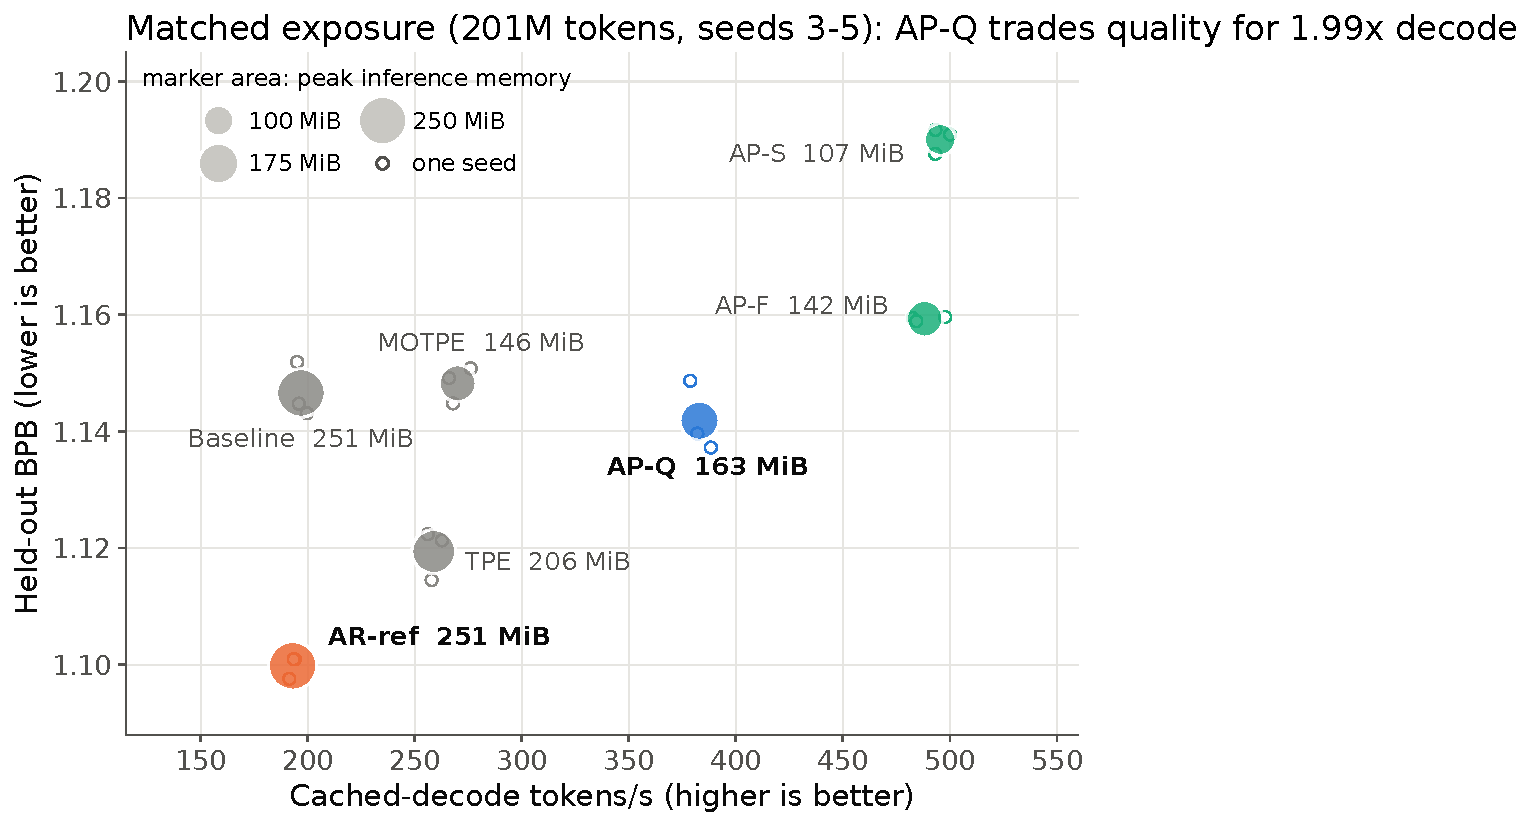
\includegraphics[width=\linewidth]{../poster_figures/cr_pareto.pdf}
\end{minipage}
\end{panel}
\end{minipage}\hfill
% ---------------------------------------------------------------- column 3
\begin{minipage}[t]{0.305\linewidth}\vspace{0pt}
\begin{panel}{A second agent, same contract}
\raggedright Codex (\texttt{gpt-5.6-sol}, \CRCxAttempts{} attempts) and \textcolor{opus}{\textbf{Claude Opus 5.5}} (\CROpAttempts{} attempts) from the same baseline, seed, prompt and Pareto rule.\\[8pt]
\centering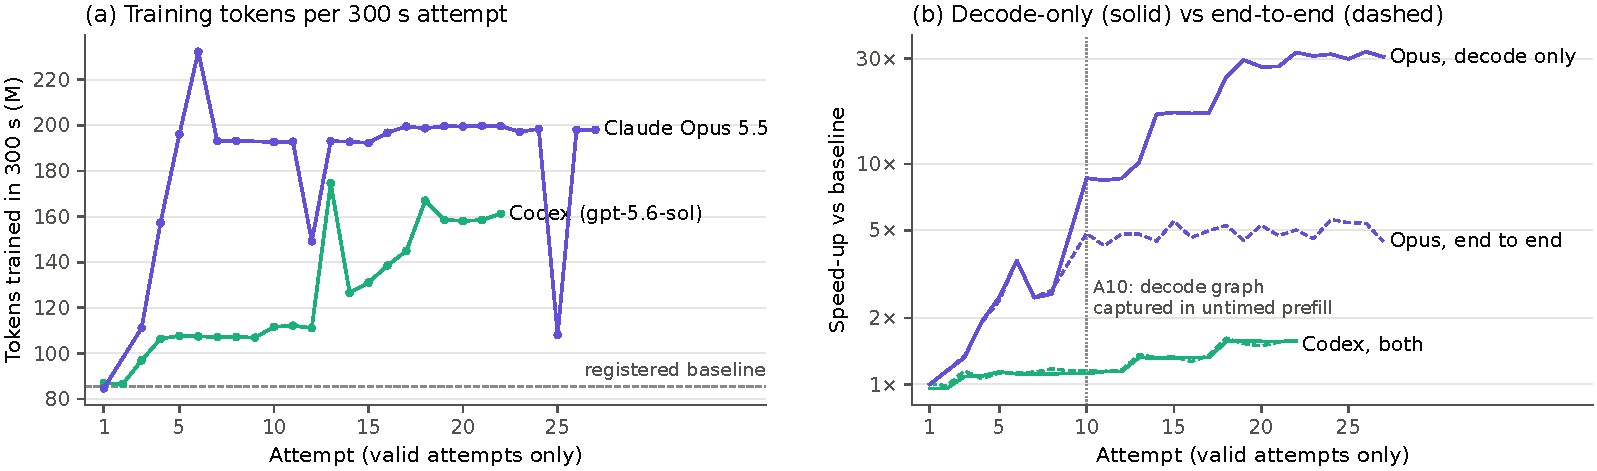
\includegraphics[width=\linewidth]{../poster_figures/cr_agents.pdf}\\[8pt]
\raggedright
\begin{itemize}\setlength{\itemsep}{4pt}
\item Both cut batch and model size to train more tokens in 300\,s (Opus: \CROpTokRatio$\times$ the baseline).
\item Opus: \statnum{opus}{\CROpDecodeLo--\CROpDecodeHi$\times$} decode-only, but only \statnum{opus}{\CROpEtoELo--\CROpEtoEHi$\times$} end to end: from attempt \CROpAdapterAttempt{} its adapter captured the decode graph inside the \textbf{untimed prefill}.
\item At $\approx$ matched tokens Opus is again worse than AR-ref (held-out \CROpHeldLo--\CROpHeldHi{} vs \CROpARHeld).
\end{itemize}
\end{panel}
\vspace{18pt}
\begin{panel}{Takeaways}
\begin{itemize}\setlength{\itemsep}{6pt}
\item \textbf{The contract decides who wins.} Under fixed time, faster training buys tokens; matched exposure removes that.
\item \textbf{Agents optimise what is timed.} Report decode-only next to end-to-end.
\item \textbf{Contract card:} stopping rule, seeds, tokens/updates/FLOPs, throughput variance, what each metric times, selection funnel, harness invariants.
\end{itemize}
\end{panel}
\end{minipage}
\end{document}
